\section{Generative Models}
	discriminative vs generative.
	
	Objectives:
	
	learn $p_{model}(x)$ that approximates $p_{data}(x)$.换言之假设image$ \in \mathcal{X} = \mathcal{R}^{3\times H \times W}\sim p_{data}$.我们想要习得这个分布.
	
	隐式和显式.
	
	本门课接触三个生成模型:pixelRnn, , gan
	
	expilcity density model, or Fully Visible Belief Network (FVBN)
	
	假设我们的隐式概率模型是$p(x) = p(x_1, \cdots, x_n)$.这一步没有引入任何信息.应用链式法则可得:
	
	\begin{equation}
		p(x)=\prod_{i=1}^{n} p\left(x_{i} \mid x_{1}, \ldots, x_{i-1}\right)
	\end{equation}
	
	什么样的神经网络能够处理这样的连续的条件概率?(显然我们希望获得一个shared 网络)
	
	RNN.但这样有问题:首先网络太大,其次如果要截断梯度,语义不明.
	
	CNN.只依赖局部的pixel.train的时候可并行计算,因为像素已经存在.但生成仍然缓慢:必须按照顺序生成.\marginpar{\kaishu 但是凭什么认为只和上面的像素相关呢?}
	
	说实话,效果不咋地...
	
	优点:可显示表达,容易优化,采样好(?相对).缺点:慢
	
	\subsection{Approximate density:Variational Autoencoder}
	变分自动编码器?
	
	PixelRNN实际上只是非常低维的.因为只有少数取值.
	
	VAEs:
	
	\begin{equation}
		p_{\theta}(x)=\int p_{\theta}(z) p_{\theta}(x \mid z) d z
	\end{equation}
	
	如何进行学习?
	
	L2 loss和高斯噪声?为什么输出会比较糊.
	
	看起来在前面的AE当中,我们只需要decoder部分就可以完成生成.事实果真如此吗?如果只有decoder,那么z服从何种分布完全不了解(总不能是均匀分布吧).需要它的分布容易sample,不要分布太广(太过稀疏不利于网络学习).\marginpar{\kaishu 那么为什么要选用高斯分布呢?缺失没有一种原则说明哪种分布更好.}
	
	两者都容易算,但是其积分不容易计算.蒙特卡洛,维数太高.
	
	\begin{figure}[htbp]
		\centering
		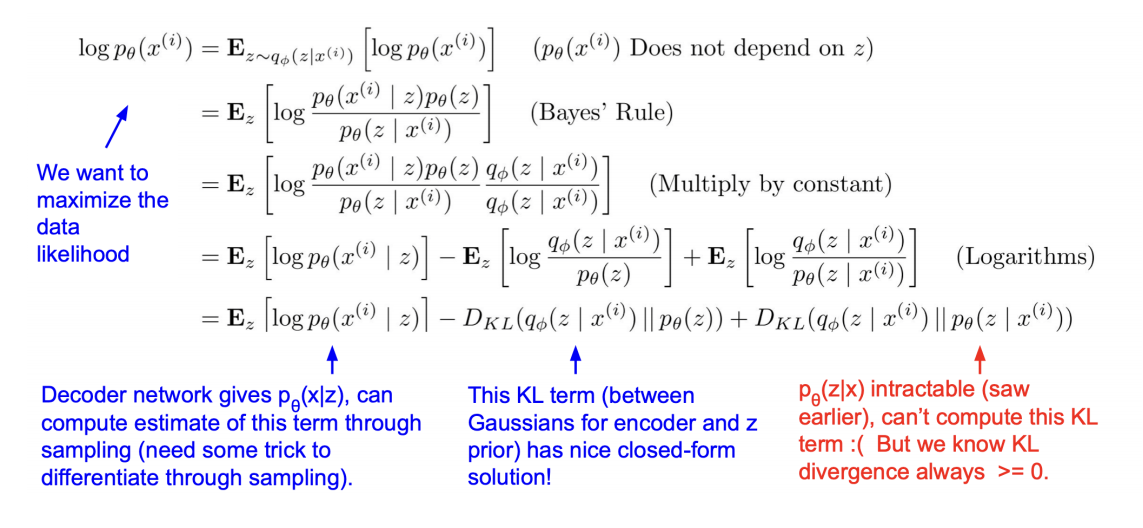
\includegraphics[scale=0.65]{figures/VAE.png}
		\caption{推导过程}
		\label{}
	\end{figure}

	
	我们此前接触的网络都是判别模型,given x, 判定y, P(X|Y).上节课介绍的生成模型,所有的变量就是$X$,我们学习$P(X)$或者$P(X|Y)$(if labels are available).本学期我们准备介绍的PixelRNN/CNN,VAE and GAN.
	
	\subsection{重学VAE}
	VAE如果有统计学习的基础,可以更容易地理解.\marginpar{\kaishu }
	
	VAE来自Auto Encoder. 我们的生成模型有一个(latent space?)中的向量$z$.一般取先验分布为$\mathcal{N}(\bm 0, \bd I)$.所有的函数都需要支持概率输出.这与AE不同,后者一般只输出一个值.那么如何从一个值变成分布呢?将输出经过一个Probabilistic model.即,你认定了它服从某种分布之后,再转换为概率分布.(比如,你认为它是高斯噪声,那么这就是你的概率模型,也就意味着你默许了生成图片中的高斯噪声.当然,你也可以选择其他概率模型.)
	
	\marginpar{\kaishu 这里我们默许了$z \sim \mathcal{N}(\bm 0, \bd I)$}
	\begin{equation}
		p_{\theta}(x)=\int p_{\theta}(z) p_{\theta}(x \mid z) d z  
	\end{equation}

	核心区别:估计mu, sigma
	
	如何计算积分?intractable.那么,MC方法可以吗?就是:
	
	\begin{equation}
		\log p(x) \approx \log \frac{1}{k} \sum_{i=1}^{k} p_{\theta}\left(x \mid z^{(i)}\right), \text { where } z^{(i)} \sim p(z)
	\end{equation}
	
	但是,我们很难在latent空间中精准地找到某张照片对应的z,因此取样的绝大多数结果都是0,效果必定差.
	
	\begin{wrapfigure}{l}{6cm}
		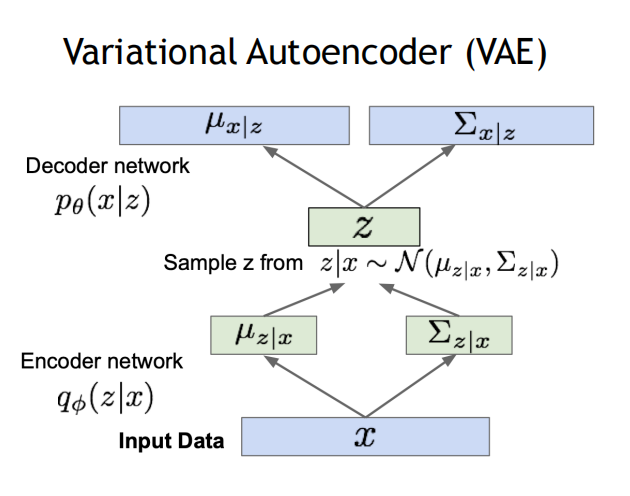
\includegraphics[scale=0.5]{figures/VAE_2.png}
		\caption{VAE结构}
	\end{wrapfigure}
	
	另一种方式:利用Bayes公式,如果能够引入后验概率$p_{\theta}(z|x)$,
	\begin{equation}
		p_{\theta}(x)=\frac{p_{\theta}(x, z)}{p_{\theta}(z \mid x)}=\frac{1}{p_{\theta}(z \mid x)} p(z) p_{\theta}(x \mid z)
	\end{equation}

	但是我们并没有从根本上解决问题.现在,我们希望学一个神经网络近似$p_{\theta}(z \mid x)$,\marginpar{\kaishu 那$p_{\theta}(x \mid z)$为啥不能学?}也就是学习一个$q_{\phi}(z|x)$来近似$p_{\theta}(z|x)$.最后我们的网络结构如图.如果是AE,那么就没有方差一项了,唯一对应,没有随机性.这里,注意$q_{\phi}$只是对$p$的近似.
	
	\clearpage
	
	\begin{equation}
		\begin{aligned}
			\log p_{\theta}\left(x^{(i)}\right) &=\mathbf{E}_{z \sim q_{\phi}\left(z \mid x^{(i)}\right)}\left[\log p_{\theta}\left(x^{(i)}\right)\right] \quad\left(p_{\theta}\left(x^{(i)}\right) \text { Does not depend on } z\right) \\
			&=\mathbf{E}_{z}\left[\log \frac{p_{\theta}\left(x^{(i)} \mid z\right) p(z)}{p_{\theta}\left(z \mid x^{(i)}\right)}\right] \quad(\text { Bayes' Rule) }\\
			&=\mathbf{E}_{z}\left[\log \frac{p_{\theta}\left(x^{(i)} \mid z\right) p(z)}{p_{\theta}\left(z \mid x^{(i)}\right)} \frac{q_{\phi}\left(z \mid x^{(i)}\right)}{q_{\phi}\left(z \mid x^{(i)}\right)}\right] \quad \text { (Multiply by constant) } \\
			&=\mathbf{E}_{z}\left[\log p_{\theta}\left(x^{(i)} \mid z\right)\right]-\mathbf{E}_{z}\left[\log \frac{q_{\phi}\left(z \mid x^{(i)}\right)}{p_{\theta}(z)}\right]+\mathbf{E}_{z}\left[\log \frac{q_{\phi}\left(z \mid x^{(i)}\right)}{p_{\theta}\left(z \mid x^{(i)}\right)}\right] \quad(\text { Logarithms }) \\
			&=\mathbf{E}_{z}\left[\log p_{\theta}\left(x^{(i)} \mid z\right)\right]-D_{K L}\left(q_{\phi}\left(z \mid x^{(i)}\right) \| p(z)\right)+D_{K L}\left(q_{\phi}\left(z \mid x^{(i)}\right) \| p_{\theta}\left(z \mid x^{(i)}\right)\right)
		\end{aligned}
	\end{equation}
	
	我们试图最大化下界,它被称为Evidence Lower BOund(ELBO).第一项最大化,也就是让网络输出的分布的theta接近真实的分布(均值接近,方差小\marginpar{\kaishu 方差变大?},那么第一项就大!另外注意上式的$x^{(i)}$并不是网络输出,而是输入.)第二项最大化,也就是希望q与p(z)接近.这是因为VAE必须知道z的分布情况,否则生成的时候很难将z取值在概率密集的部分.当然,这和我们真正的的目的还是有所偏差,因为loss的要求是将每个xi的生成的z都是Gaussian,但我们实际的意图是将所有xi构成的集合生成的z的集合满足Gaussian.\marginpar{\kaishu 所以,这有什么区别?虽然我们添加这一项希望其接近高斯,但这一项绝不可真正为0,否则就与x无关了,这样就不含x的信息了,从而不可能进行重建}.
	
	因此,VAE的loss非常有趣,它的$\phi$看似只出现在第二项,但实际上还出现在第一项的$z$里面,因此我们将$z$写成$z=\mu_{z \mid x}+\epsilon \sigma_{z \mid x}$,从而有梯度可以回传.另外,ELBO的计算也是intractable的,因为第一项的$\mathbb{E}_{z}$这一步就计算不出来,我们直接扔掉期望,取它自己作为MC的估计.
	
	那你怎么不一开始就这么干?
	
	我们说,两个被估计的量分别是$\log\xk{\mathbb{E}_z \zk{p_{\theta} \xk{x^{(i)}  \mid z}}}$和$\mathbb{E}_{z} \log p_{\theta} \xk{x^{(i)}\mid z}$,前者的$z \sim p$,后者则是q,后者实际上更加集中.而且log和期望的次序也交换了.
	
	实际上我们有时直接令$\Sigma_{x \mid z} = \bd I$.因为loss当中,形式为
	\begin{equation}
		\exp^{-\xk{\frac{x - \mu}{\sigma}}^2}
	\end{equation}
	
	最后一个问题:这东西跟变分(variational)究竟有什么关系?要说起变分,我们不得不先讲泛函\marginpar{\kaishu 同时想起了我学得极差的数理方法和更差的数学分析}.泛函简单地说就是函数的函数,或广义的函数.变分,是指自变量\textbf{函数}发生的变化,为与自变量的变化$\dd x$区分,我们一般用$\delta$表示.例如我们想要求解空间中$A, B$两点之间最短的曲线,设任意一条曲线为$f(x, y)$,其长度为
	\begin{equation}
		l = \int_{A}^{B} f(x,  y) \dd s.
	\end{equation}

	当自变量函数$f$发生微小变化$\delta f$时,长度也发生了$\delta l$的变化.运用EL方程,我们可以求得
	\begin{equation}
		\frac{\delta l}{\delta f} = 0
	\end{equation}
	时的函数$f$.
	
	在VAE当中,我们实际上也是希望找到$q_\theta$来近似$p_{\theta}$,也是变分的过程.但是实际上我们并没有使用任何变分法的技术,因为我们已经加入了先验的知识进行参数化,从而将搜索空间限制为$\theta$上,而非无限维的函数空间.
	
	
	\subsection{VAE}
	
	前面我们曾经讲过AutoEncoder的概念,其实它可以视为一种降维手段,将原数据通过一定处理(如多层神经网络)获得其另一种表示(或称编码),这个过程就是encode,然后需要时可以进行解码恢复.它本质上可以视为学习两个映射:
	\begin{equation}
		\begin{array}{l}
			\phi: \mathcal{X} \rightarrow \mathcal{F} \\
			\psi: \mathcal{F} \rightarrow \mathcal{X} \\
			\phi, \psi=\underset{\phi, \psi}{\arg \min }\|\mathcal{X}-(\psi \circ \phi) \mathcal{X}\|^{2}
		\end{array}
	\end{equation}
	
	在这一节我们要讲述的VAE也是一种AutoEncoder,只不过它引入了一些概率上的内容,编码解码不再是一一对应的,而是服从一些概率分布.具体来说,\marginpar{\kaishu 这里的$\bm X, \bm Z$都可能是随机向量.}我们有一些对$\bm X$观测而得到的量$\bm x_i, i = 1, 2, \cdots, n$, 我们希望将其进行编码之后,得到由另一些变量表示的形式,后者被称为隐变量(latent variable).然后我们希望再从这些隐变量中恢复得到服从$\bm X$分布的量.也就是说,我们希望从$\bm X$的一些观测值出发,试图用一些其他的变量$\bm Z$(即隐变量)描述这个量的概率分布,这样我们就\textbf{间接}习得了$\bm X$的分布$p(\bm X)$,同时我们还要给出$\bm Z$服从的分布$q(\bm Z)$,这样我们就可以依据分布$q$选取另外的$\bm Z$,然后通过解码来生成一些新的$\bm x_j$,后者仍然服从$\bm X$的分布,但是我们此前没有见过的,此时解码器就变成了一个关于$\bm X$的生成模型.
	
	我们整理一下上面的内容,假设所有已知数据$\bm x$来自一个未知的概率分布$P(\bm x)$,我们希望用一组参数$\theta$来确定一个参数分布$p_{\theta}(\bm x)$来拟合$P(\bm x)$.我们假定$\bm x$与另一些隐变量$\bm z$有关,那么依据边缘分布和条件分布的相关性质可知
	\begin{equation}
		p_{\theta}(\bm x) = \int_{\bm z} p_\theta(\bm x, \bm z) \dd \bm z = \int_{\bm z} p_\theta(\bm x\mid \bm z) p_{\theta}(\bm z) \dd \bm z
	\end{equation}

	这里$p(\bm z)$一般被称为先验分布,一般取其为标准正态分布\marginpar{\kaishu 正因为$\bm z$是先验的,所以$p_{\theta}(\bm z)$也可以写成$p(\bm z)$,因为它没有参数.}.而$p_{\theta}(\bm z \mid \bm x)$则被称为后验分布.编码器学习的就是$p_{\theta}(\bm z \mid \bm x)$, 因为它代表了如何从$\bm x$转换到隐变量.解码器学习的则是$p_{\theta}(\bm x \mid \bm z)$.
	
	上式并不能解决我们的问题.尽管我们确定了先验分布,而且$p_{\theta}(\bm x \mid \bm z)$可由解码器学习,但上式的积分是难以计算的,因为实际操作中我们不可能遍历$\bm z$所在的高维空间.所以我们试图用贝叶斯公式曲线救国:
	
	\begin{equation}
		p_{\theta}(\bm x) = \frac{p_\theta(\bm x\mid \bm z) p(\bm z)}{p_\theta(\bm z\mid \bm x)}
	\end{equation}

	那么$p_\theta(\bm z\mid \bm x)$又怎么获得呢?这其实是编码器负责学习的分布,\marginpar{\kaishu 这可能就是神经网络之道:凡是不容易算不好表示的东西,通通丢给神经网络去学习...}因此我们用编码器来学习它.我们记编码器学习的分布为$q_\phi(\bm z\mid \bm x)$.
	
	那么如何度量学习的好坏呢?我们知道两个分布的差异可以用KL-divergence度量.
	
	最后我们用一句话来概括VAE的工作,然后进入形式化的推导:在VAE当中,输入数据$\bm X$是来自于一个特定的先验参数分布$p_{\theta}(\bm x)$,随后我们同时训练encoder和decoder,使得在我们学习的后验分布$q_\phi(\bm z\mid \bm x)$和真实后验分布$p_\theta(\bm z\mid \bm x)$的KL散度$\operatorname{D_{KL}}(q_\phi \parallel p_\theta)$作为度量之下的重建误差最小.
	
	\subsubsection{ELBO}
	计算学习的后验分布$q_\phi(\bm z\mid \bm x)$和真实后验分布$p_\theta(\bm z\mid \bm x)$的KL散度$\operatorname{D_{KL}}(q_\phi \parallel p_\theta)$得到:
	\begin{equation}
		\begin{aligned}
			\operatorname{D_{KL}}\left(q_{\phi}(\bm{z} \mid \bm{x}) \| p_{\theta}(\bm{z} \mid \bm{x})\right) &=\int q_{\phi}(\bm{z} \mid \bm{x}) \log \frac{q_{\phi}(\bm{z} \mid \bm{x})}{p_{\theta}(\bm{z} \mid \bm{x})} \dd \bm{z} \\
			&=\int q_{\phi}(\bm{z} \mid \bm{x}) \log \frac{q_{\phi}(\bm{z} \mid \bm{x}) p_{\theta}(\bm{x})}{p_{\theta}(\bm{z}, \bm{x})} \dd \bm{z} \\
			&=\int q_{\phi}(\bm{z} \mid \bm{x})\left(\log \left(p_{\theta}(\bm{x})\right)+\log \frac{q_{\phi}(\bm{z} \mid \bm{x})}{p_{\theta}(\bm{z}, \bm{x})}\right) \dd \bm{z} \\
			&=\log \left(p_{\theta}(\bm{x})\right)+\int q_{\phi}(\bm{z} \mid \bm{x}) \log \frac{q_{\phi}(\bm{z} \mid \bm{x})}{p_{\theta}(\bm{z}, \bm{x})} \dd \bm{z} \\
			&=\log \left(p_{\theta}(\bm{x})\right)+\int q_{\phi}(\bm{z} \mid \bm{x}) \log \frac{q_{\phi}(\bm{z} \mid \bm{x})}{p_{\theta}(\bm{x} \mid \dd \bm{z}) p_{\theta}(\bm{z})} \dd \bm{z} \\
			&=\log \left(p_{\theta}(\bm{x})\right)+E_{\bm{z} \sim q_{\phi}(\bm{z} \mid \bm{x})}\left(\log \frac{q_{\phi}(\bm{z} \mid \bm{x})}{p_{\theta}(\bm{z})}-\log \left(p_{\theta}(\bm{x} \mid  \bm{z})\right)\right) \\
			&=\log \left(p_{\theta}(\bm{x})\right)+\operatorname{D_{KL}}\left(q_{\phi}(\bm{z} \mid \bm{x}) \| p_{\theta}(\bm{z})\right)-\mathbb E_{\bm{z} \sim q_{\phi}(\bm{z} \mid \bm{x})}\left(\log \left(p_{\theta}(\bm{x} \mid \bm{z})\right)\right)
		\end{aligned}
	\end{equation}
	
	将上式重写成
	\begin{equation}
		\log \left(p_{\theta}(\bm{x})\right) - \operatorname{D_{KL}}\left(q_{\phi}(\bm{z} \mid \bm{x}) \| p_{\theta}(\bm{z} \mid \bm{x})\right) = -\operatorname{D_{KL}}\left(q_{\phi}(\bm{z} \mid \bm{x}) \| p_{\theta}(\bm{z})\right)+\mathbb E_{\bm{z} \sim q_{\phi}(\bm{z} \mid \bm{x})}\left(\log \left(p_{\theta}(\bm{x} \mid \bm{z})\right)\right)
	\end{equation}
	
	左侧第一项是我们希望最大化的输出的概率,第二项是希望最小化的分布差异,综合起来应该最大化左侧.我们再来看右侧,第一项是$q_{\phi}(\bm{z} \mid \bm{x})$和$p(\bm z)$之间的KL散度,最小化这一项说明我们希望后验分布也符合正态.最后一项最大化则是希望我们的解码器预测更加准确.使用优化理论的常用手段,我们将损失函数定义为
	\begin{equation}
		\mathcal{L}_{\theta, \phi} = -RHS = \operatorname{D_{KL}}\left(q_{\phi}(\bm{z} \mid \bm{x}) \| p_{\theta}(\bm{z})\right)-\mathbb E_{\bm{z} \sim q_{\phi}(\bm{z} \mid \bm{x})}\left(\log \left(p_{\theta}(\bm{x} \mid \bm{z})\right)\right)
	\end{equation}

	我们希望求得
	\begin{equation}
		\theta^{*}, \phi^{*} = \arg\min_{\theta, \phi} \mathcal{L}_{\theta, \phi}
	\end{equation}

	现在我们来看看这两项具体如何运算.第一项,由于我们假定后验分布也是高斯分布,两个高斯分布的KL散度有闭式解\marginpar{\kaishu 因为我们假定后验分布的隐变量彼此独立,即$\bm \Sigma = \diag \{ \sigma_1^2, \cdots, \sigma_d^2\}$, 因此多维的情形可以由一维计算后求和.计算过程略.}
	
	\begin{equation}
		\operatorname{D_{KL}}(p(\bm z \mid \bm x) \| q(\bm z))=\frac{1}{2} \sum_{k=1}^{d}\left(\mu_{(k)}^{2}(x)+\sigma_{(k)}^{2}(x)-\ln \sigma_{(k)}^{2}(x)-1\right)
	\end{equation}
	
	对于后验分布,我们有
	\begin{equation}
		q(\bm x \mid \bm z)=\frac{1}{\prod_{k=1}^{D} \sqrt{2 \pi \tilde{\sigma}_{(k)}^{2}(\bm z)}} \exp \left(-\frac{1}{2}\left\|\frac{\bm x-\tilde{\mu}(\bm z)}{\tilde{\sigma}(\bm z)}\right\|^{2}\right)
	\end{equation}

	得到
	\begin{equation}
		-\ln q(\bm x \mid \bm z)=\frac{1}{2}\left\|\frac{\bm x-\tilde{\mu}(\bm z)}{\tilde{\sigma}(\bm z)}\right\|^{2}+\frac{D}{2} \ln 2 \pi+\frac{1}{2} \sum_{k=1}^{D} \ln \tilde{\sigma}_{(k)}^{2}(\bm z)
	\end{equation}

	这里我们常常令$\sigma_i = 1$,即协方差矩阵为单位阵.否则对于上面这一项,网络可以通过一直增大方差的方式来减小loss.此时损失函数就变为MSE.\marginpar{\kaishu 算了,还是看参考文献\cite{kexuefm-autoencoder}吧.}
	
	\clearpage
	
	